%----------------------------------------------------------------------
\section[Simulador de Vuelo]{Simulador de Vuelo: Tecnam-P92}
%----------------------------------------------------------------------

%----------------------------------------------------------------------
\paragraph{Descripción y objetivo}
%----------------------------------------------------------------------

El proyecto consistió en el diseño, desarrollo y construcción de un simulador de vuelo basado en el avión Tecnam-P92, utilizado por la escuela de vuelo del Aeroclub de Castellón. El principal objetivo del simulador fue servir de ayuda en el entrenamiento de procedimientos y vuelos VFR para todos los alumnos de la escuela (entre los que el autor formó parte).2

\begin{wrapfigure}{r}{0.5\linewidth}
	\centering
	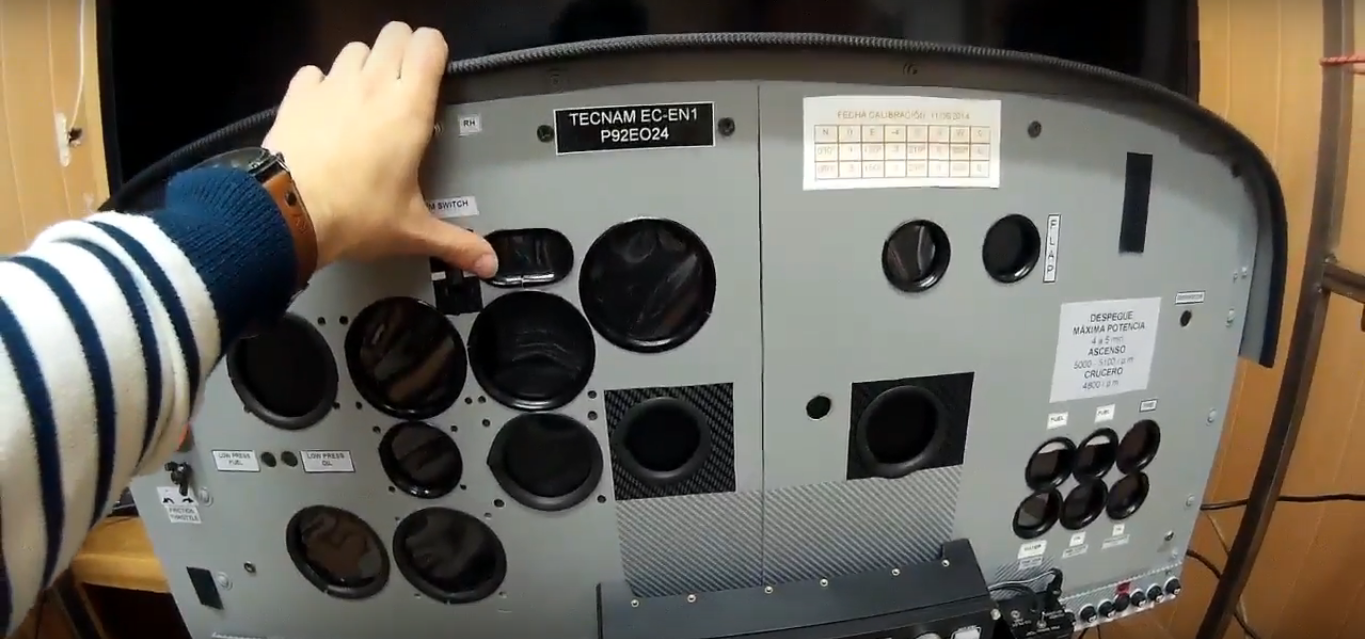
\includegraphics[width=0.5\textwidth]{simulador.png}
	\caption*{Simulador de vuelo del P92}
	\label{labelformat=empty}
\end{wrapfigure}

\paragraph{Diseño, desarrollo y construcción}

El simulador se diseñó y construyó tratando de aportar el máximo realismo a la vez que se optimizaron los costes de material. Para su construcción se emplearon tres pantallas de 42 pulgadas cada una que envuelven al usuario y lo sumergen dentro de ese entorno virtual. El panel de instrumentos, construido en MDF, esconde una cuarta pantalla que proyecta los instrumentos de vuelo principales, igual a los que se pueden encontrar en el avión de escuela. Finalmente, el usuario puede sentarse a practicar el vuelo virtual en una asiento que incluye incluso un cinturón de seguridad, pues a pesar de no ser necesario, su uso es imprescindible en el vuelo real y por ello se optó por su instalación en el simulador.

\paragraph{Interacción de los componentes con el simulador}
El simulador cuenta con una gran variedad de componentes electrónicos de todo tipo: interruptores, pulsadores, selectores, potenciómetros... Su función es recrear los componentes que el piloto puede encontrar en la aeronave original. Todos ellos son gobernados por un microcontrolador Arduino, que mediante la interfaz gratuita de "LINK2FS", permite la comunicación con el software "Microsoft Flight Simulator X". La gran mayoría de interruptores y pulsadores fueron reciclados, pero cumplen a la perfección su función.

\begin{wrapfigure}{r}{0.5\linewidth}
	\centering
	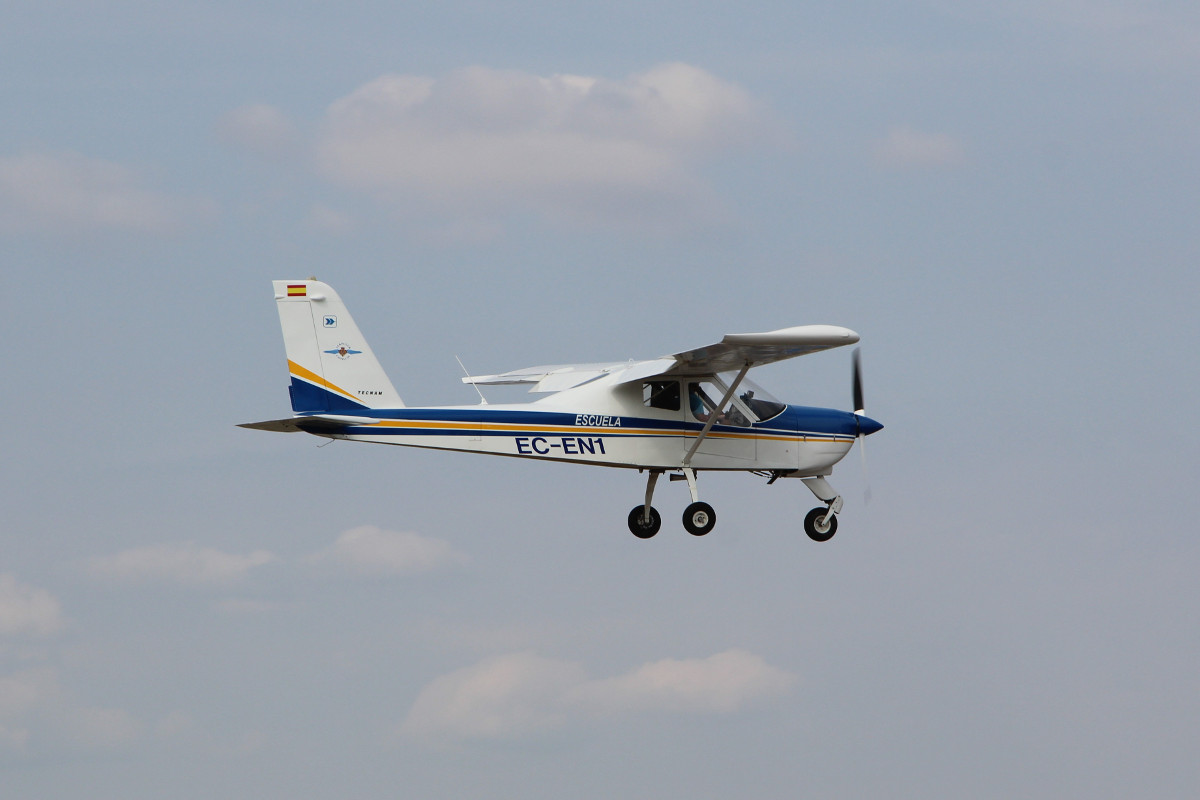
\includegraphics[width=0.5\textwidth]{tecnam.jpg}
	\caption*{Tecnam-P92 del Aeroclub de Castellón}
	\label{labelformat=empty}
\end{wrapfigure}

\paragraph{Realismo del software}
Durante los últimos años, la comunidad relacionada con la aviación y el vuelo virtual ha ido creciendo. Ello se debe principalmente a la reducción de costes de los equipos informáticos y el auge de la industria de los videojuegos. Muchos son los que se dedican, como el autor, a realizar aportes a la comunidad de forma totalmente gratuita y desinteresada. Uno de los "add-ons" más conocidos y que se decidió utilizar en el simulador fue el "Real Spain". Un conjunto de texturas foto-realistas que permiten la simulación del vuelo VFR con una calidad increíble.

\paragraph{A día de hoy} El simulador continúa en el Aeroclub de Castellón y algunos socios lo utilizan para practicar vuelos, generalmente relacionados con los ANR (Air Navigation Race) y así ahorrar costes en horas de vuelo.



